\documentclass[tikz, border=10pt]{standalone}
\usepackage{pgfplots}
\usepackage{amsmath}
\usetikzlibrary{backgrounds}
\pgfplotsset{compat=1.18}

\begin{document}
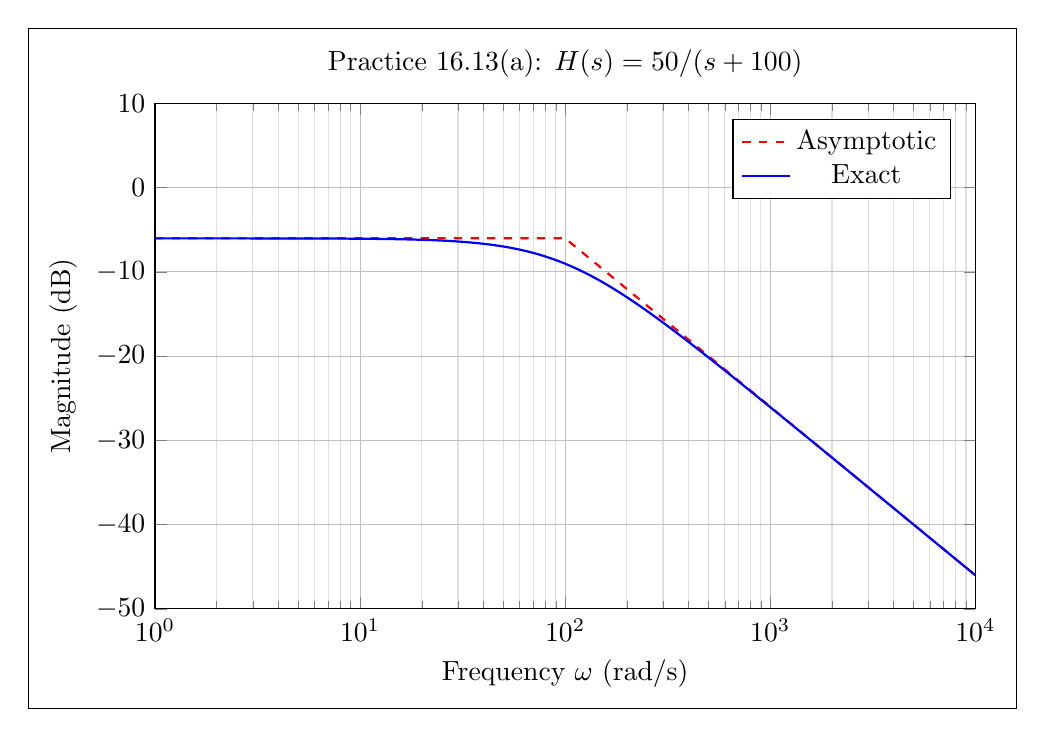
\begin{tikzpicture}[show background rectangle]
    \begin{semilogxaxis}[
        width=12cm, height=8cm,
        title={Practice 16.13(a): $H(s) = 50/(s + 100)$},
        xlabel={Frequency $\omega$ (rad/s)},
        ylabel={Magnitude (dB)},
        grid=both,
        xmin=1, xmax=10000,
        ymin=-50, ymax=10,
        minor grid style={gray!25},
        major grid style={gray!50},
        legend pos=north east,
    ]

    % H(s) = 50/(s+100) = 0.5/(1 + s/100)
    % K = 0.5 => -6.02 dB
    % Pole at 100 => Break freq 100 rad/s
    
    % Asymptote
    \addplot[red, dashed, thick] coordinates {
        (1, -6.02) (100, -6.02) (10000, -46.02) 
    };
    \addlegendentry{Asymptotic}

    % Exact
    % 20*log10( 50 / sqrt(100^2 + x^2) )
    \addplot[blue, thick, domain=1:10000, samples=200] {20*log10(50/sqrt(10000 + x^2))};
    \addlegendentry{Exact}
    
    \end{semilogxaxis}
\end{tikzpicture}
\end{document}
